\section{Literature Review}
\label{sec:literature}
We discuss literature organised into several key elements; starting with an overview of the variety of sensors used for HAR; to different datasets that are available for model generation; analyse deep learning architectures; and paradigms suited to learning from multi-modal data streams. 

\subsection{Sensors}
\label{sec:sensors}
In the context of HAR, \citeasnoun{wang2017deep} lists three main modalities of sensors as body-worn , object and ambient sensors. Inertial sensors such as accelerometers and gyroscopes are examples of body worn sensors; whilst object sensors are those that are commonly mounted on an object to record movement or a sensor which observes a specific object. Here inertial sensors and cameras (RGBD/Depth) can be used as object sensors.Pressure sensors and temperature sensors are examples of ambient sensors where object/human interactions are sensed in a restricted area. For instance a surface can have many pressure sensor points which generate a sequence of heat-maps for pressure changes over time. Considering data generated by sensors, we can observe that wearable typically generate time-series data along several axes. For instance an accelerometer records acceleration of the subject along three axes. Sensors such as a pressure mats and depth cameras also generate time series data, but these are captured as images. 
When multi-modalities are used to capture sensor data synchronously in real-time (such as in bespoke hybrid sensors in smart home environments) the challenge for model learning is to generate data representations that enable the utilisation of all modalities and the effective fusion strategies to improve recognition accuracy for HAR.

\begin{table}
\caption{HAR datasets (A=Accelerometer, G=Gyroscope, M=Magnetometer, OS=Object Sensors, AS=Ambient Sensors, P=Pressure sensors) }
\label{table:data}
\begin{center}
\begin{tabular}{|c|c|c|c|c|} 
 \hline
 Dataset & Type & Subjects & Sensors & Classes \\
 \hline
 \citeasnoun{chen2015deep} & HAR &100 &A &8 \\
 \hline
 \citeasnoun{stisen2015smart} & HAR &9 &A and G &6 \\
 \hline
 \citeasnoun{bulling2014tutorial} & Gesture &2 &A and G &12 \\
 \hline
 \citeasnoun{chavarriaga2013opportunity} & ADL &4 &A, G, M, OS and AS &16\\
 \hline
 \citeasnoun{sundholm2014smart} & Sport Exercises &7 &P &10 \\
 \hline
\end{tabular}
\end{center}
\end{table}

Validation of HAR models in machine learning typically require datasets both for model generation and testing. Table \ref{table:data} summarises datasets used in recent HAR research. 
A notable difference is the dataset complied by \citeasnoun{chavarriaga2013opportunity} for Hierarchical Activity Inference (HAI), which allows the exploration of quality assessment applied to primitive action levels found in Activities of Daily Living (ADL). 
Unfortunately such primitives are not directly applicable for exercise recognition due to two reasons:
\begin{itemize}
\item sensor placements on limbs result in higher degrees of freedom and as such are not best placed to capture body movements in exercises as compared to ADL; 
\item the requirement for slower and controlled movement capture with exercises (certainly for MSDs) 
and the inherent characteristic of them consisting of longer sequences of sub-movements instead of shorter infrequent and non-repetitive movements as in ADL; and  
\item the need to capture greater floor surface with exercises further differentiates it from ADL calling for different types of sensing (e.g. pressure).  
\end{itemize}
When implementing reasoning models for sensing, these characteristics of exercises provide valuable insights that are not the focus of the the ADL dataset. Therefore in the context of multi-modal exercise recognition there is a clear need to capture and create new datasets to enable the advancement of exercise recognition research. 

\subsection{Deep Learning Models}
Advancement of computational power has enabled machine learning to evolve in to deep learning techniques. Deep learning models learn spatial and temporal dependencies in different abstraction levels given abundant data and has importantly eliminated the need for hand crafted features from raw data. Interestingly the model learning is closely coupled with the tuning of features that are being engineered. 

\subsubsection{Convolutional Neural Networks (CNNs)}\mbox{}\\
CNNs have demonstrated ability to learn spatial features and has been successfully applied in image classification, recommender systems and natural language processing. A convolution function extracts latent spatial dependencies in the input and organised in to feature maps. These feature maps can be viewed as creating new features through non-linear combinations of the raw input features. With increasing layers, extracted features enable the discovery of features that are increasingly conceptual in nature. 
Other aggregation operations are also included to generate layers, such as using the pooling functions, to reduce the spatial dimensions. Repeating these two operations provide feature embeddings in different abstraction levels providing the new features for classification or regression tasks (Figure \ref{fig:cnn}). 

\begin{figure}[ht]
\centering
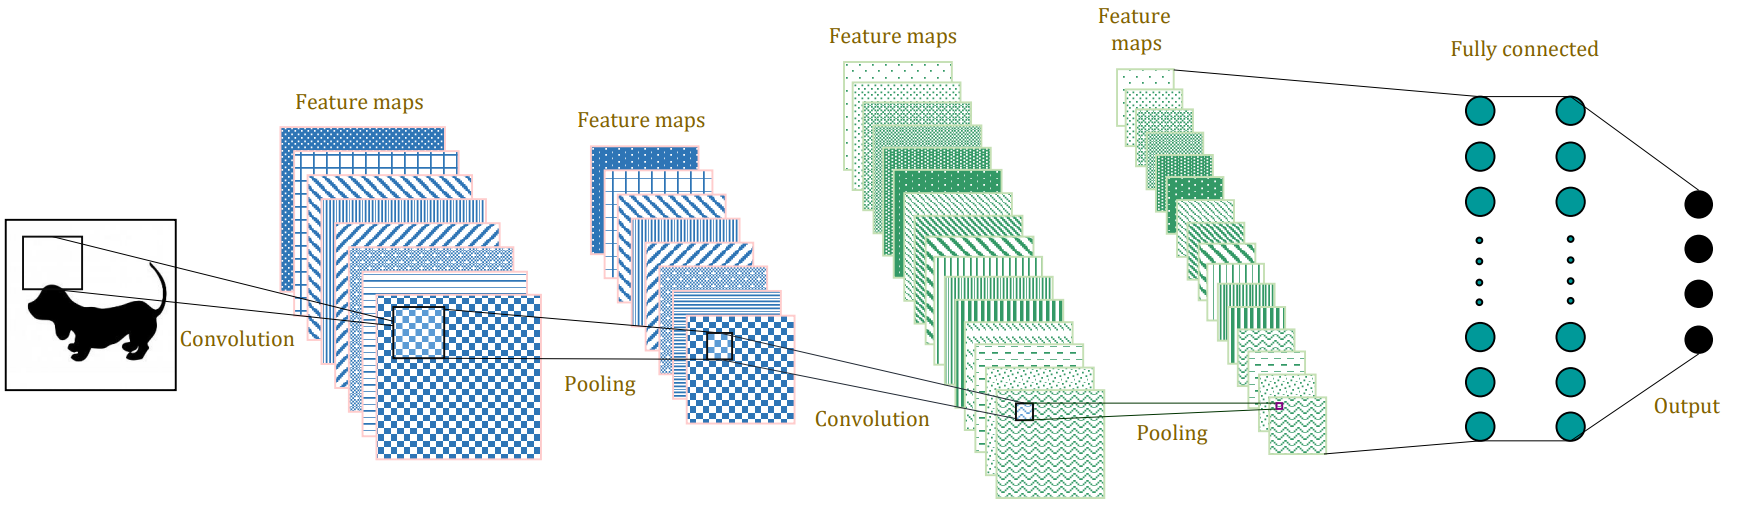
\includegraphics[width=0.8\textwidth]{cnn}
\caption{CNN with two convolution layers, second layer is a feature embedding used for the classification task}
\label{fig:cnn}
\end{figure}

\subsubsection{Recurrent Neural Networks (RNNs)} \mbox{}\\
RNNs learn dynamic temporal dependencies in data and have been applied successfully with time-series predictions, speech recognition and language translation. The Elman RNN cell (Figure \ref{fig:rnn}) is one of the basic implementations that demonstrate how RNN cell incorporates knowledge from previous time-stamp \cite{elman1990finding}. Unlike a CNN, this architecture focuses on retaining some memory of the recent learning session to influence the learning of the next iteration. Many advanced variations of RNN have been introduced since; such as LSTM, GRU and Bi-directional RNN \cite{chung2014empirical,schuster1997bidirectional}. 

Figure \ref{fig:rnn} illustrates the typical architecture of an RNN and the use of recurrence edges to introduce dependencies between time-stamps. With HAR data consisting of time dependant data, it makes sense to explore how these architectures compare with CNNs. Specifically we will explore whether the sophisticated convolutional feature embeddings can benefit from time dependant relationships that are discovered by RNNs.

\begin{figure}[ht]
\centering
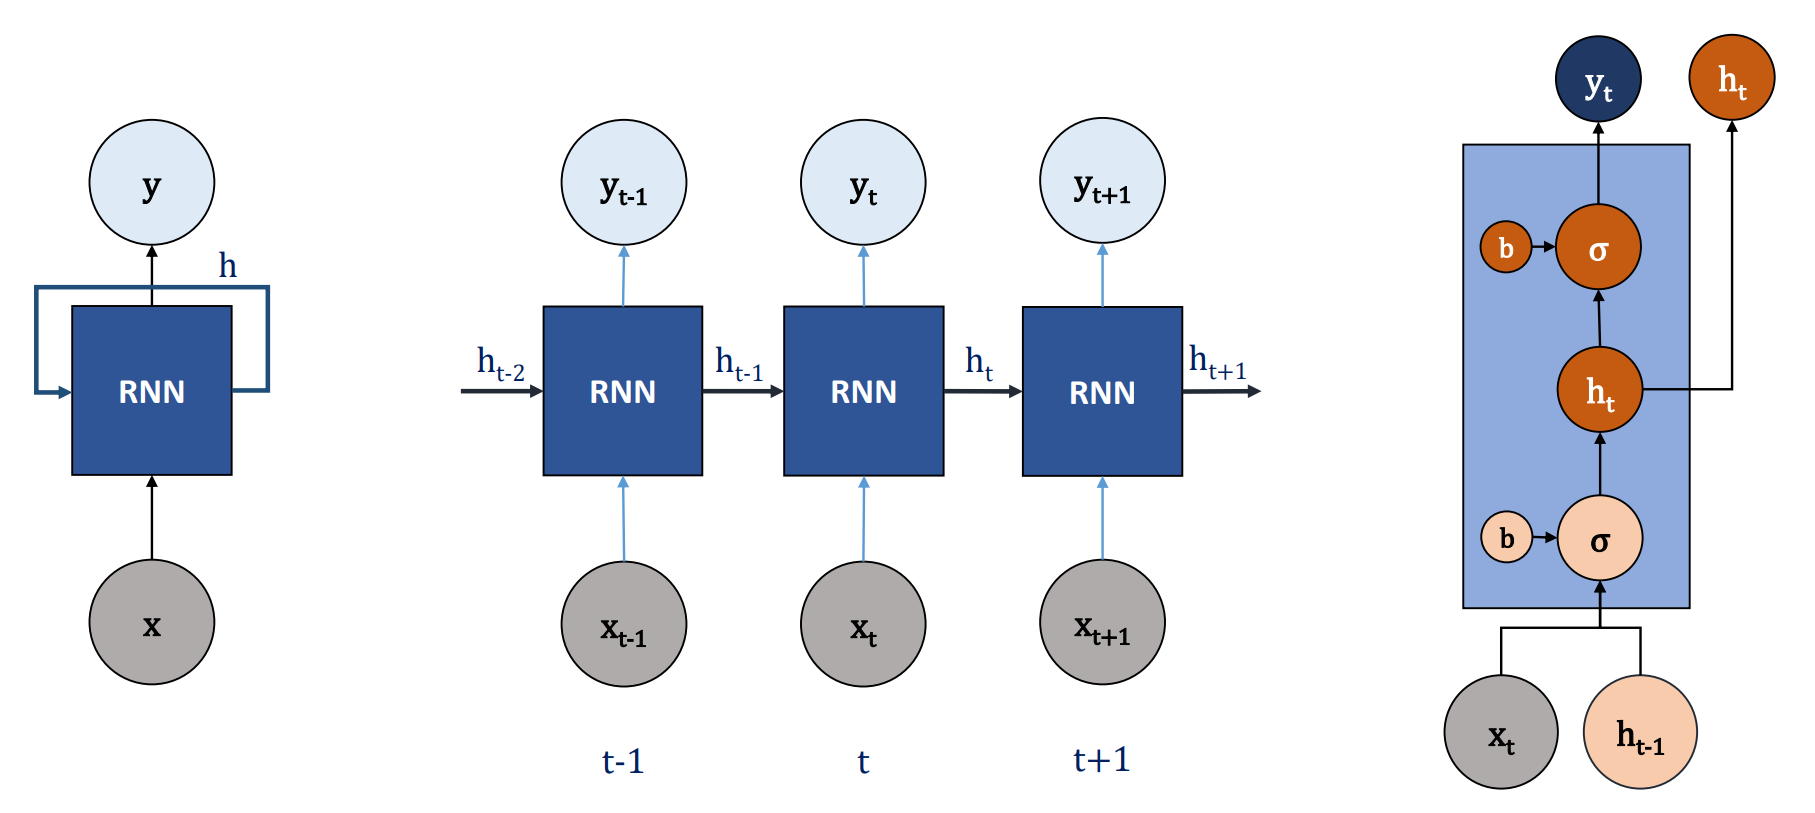
\includegraphics[width=0.7\textwidth]{rnn}
\caption{Recurrent Neural network, left: Simple RNN network, centre: RNN unfolding over time, right: Elman RNN cell}
\label{fig:rnn}
\end{figure} 

\subsubsection{Siamese Neural Networks (SNNs)} \mbox{}\\
\citeasnoun{chopra2005learning} introduced SNN as a neural network architecture that learn complex similarity metrics. Given two inputs, labelled as imposter or genuine, top layer of SNN generates a feature representation for each input that emphasises their similarity or dissimilarity. An interesting aspect of this architecture is that it enables the learning of metric space which in turn can be used to compare instances. \citeasnoun{chopra2005learning} employs SNNs for face verification tasks where CNNs build feature embeddings. We are interested in building comparable feature embeddings with spatio-temporal data from sensors which forms a novel application domain for SNNs.

\subsubsection{Auto-encoders} \mbox{}\\
\citeasnoun{hinton2006reducing} introduced the Auto-encoder (AE) as a multi-layer neural network with usually a single small central layer, where input is reconstructed at the output. The goal was to learn low-dimensional representation of the input data at the small central layer. First half of the network transforms input (encode) from high-dimensional data to low-dimensional encoding and second half of the network attempts to reconstruct data (decode) from low-dimensional encoding back to its original dimensionality. AE can be as simple as a shallow fully connected network or a complex CNN (Figure:\ref{fig:ae}) depending on the type of data being learnt by the model.
AE are known for learning from noisy data \cite{vincent2010stacked} where the network learns from noisy input and attempts to reconstruct a de-noised output. Ability of AE to rebuild an input is an interesting approach to synthesising sensor data given our requirement to operate robustly even in circumstances of absent sensors.

\begin{figure}[ht]
\centering
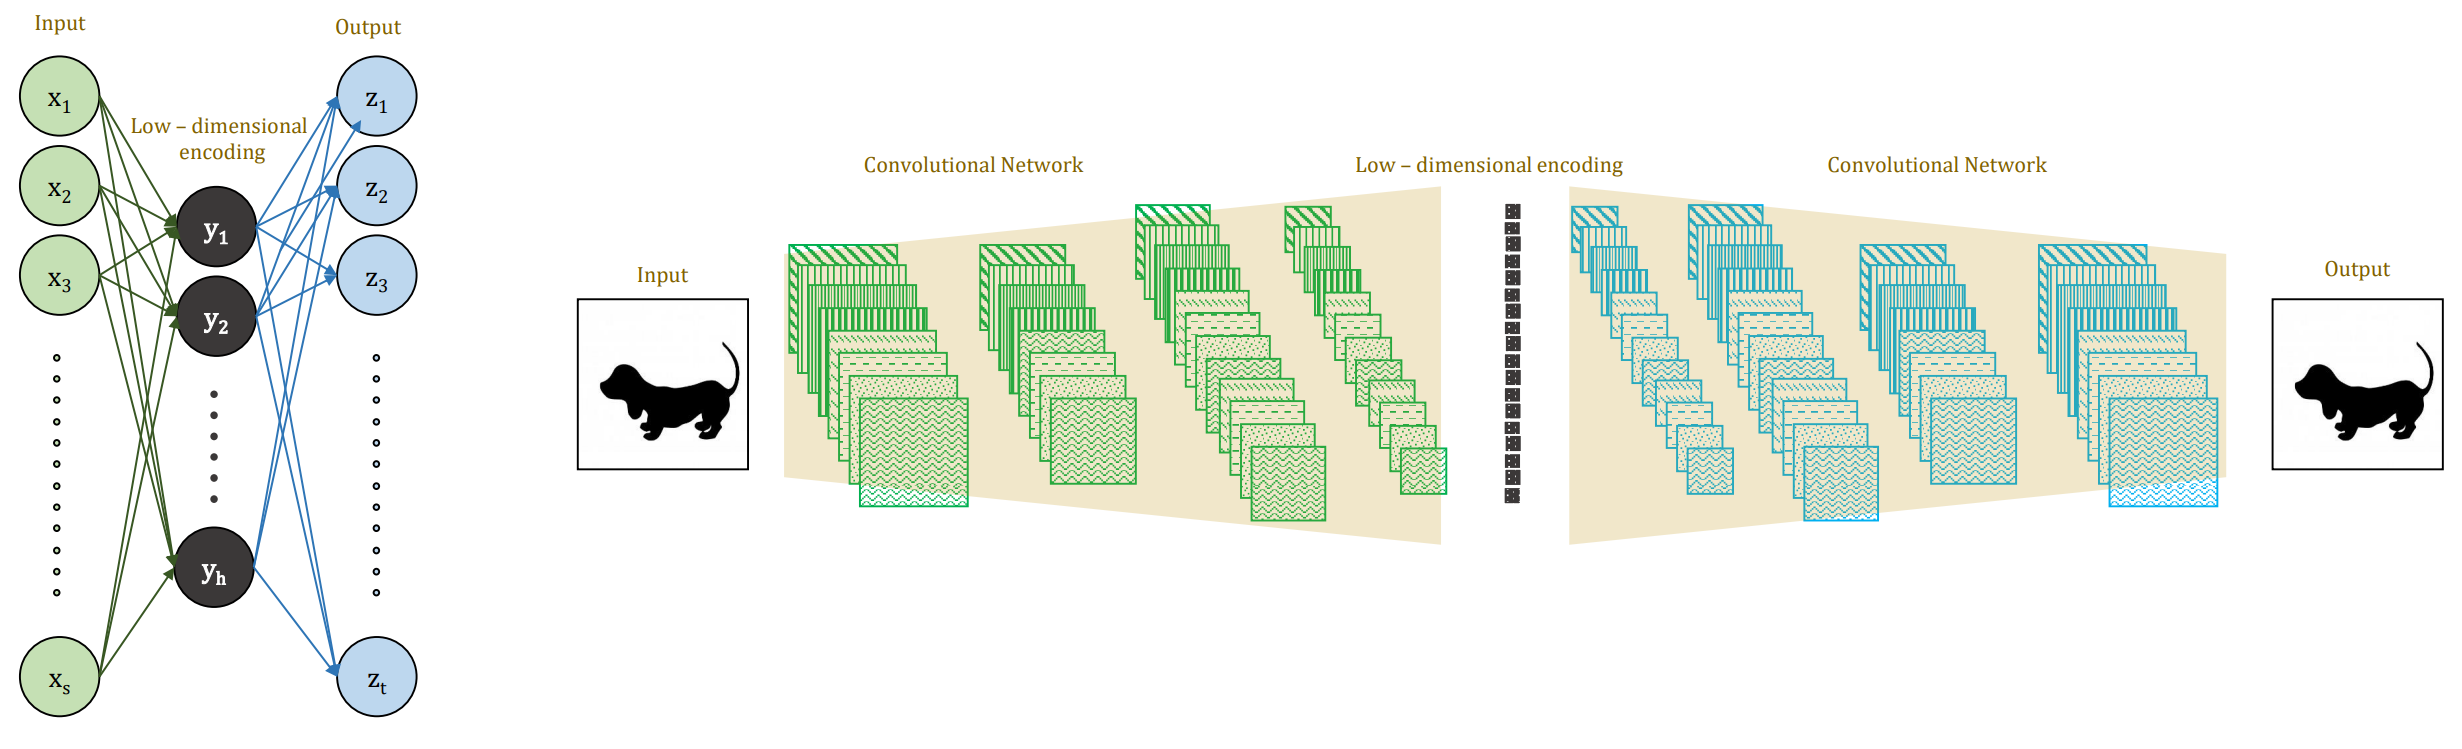
\includegraphics[width=1.0\textwidth]{autencoder}
\caption{Auto-encoders left: Shallow fully connected Auto-encoder, right: Deep Convolutional Auto-encoder }
\label{fig:ae}
\end{figure}

\subsection{Reasoning with sensors}

Early research suggests using machine learning models for activity classification needed feature engineering as a pre-processing stage. Features were extracted and refined from raw data using techniques such as Discrete Fourier Transform (DFT) and Principle Component Analysis (PCA). For instance \citeasnoun{garcia2011statistical} has used PCA to extract features from accelerometer and heart-rate data to perform Physical Activity Intensity classification; for a detailed discussion and comparative study of feature extraction methods the reader is refereed to \citeasnoun{preece2009comparison}. 

One of the main draw backs with employing hand-crafted features is that it requires several refinements using processes that are often decoupled from the model learning process. This often leads to features that remain domain specific where complex relationships are often not discovered making them less generalisable and transferable to new domains.

\subsubsection{Deep Learning Models in HAR}
The ability to engineer features as an integral part of model learning is a key advantage that deep learners have over traditional learning algorithms.
Specifically with time series data, 
\citeasnoun{ronao2016human} found that the input from two sensors can be used as different channels to the model. Their research shows that while CNN was seen to outperform traditional machine learning techniques with hand-crafted features, the hybrid approach of using temporal fast Fourier transform (tFFT) features with the CNN had resulted in the best performance. This research shows that hybrid approaches that combine both hand-crafted and learnt features lead to significant gains in HAR performance.

\citeasnoun{sani2017learning} is another notable research study involving accelerometer data from two body worn sensors on wrist and thigh. They implement a pyramid like CNN architecture in contrast to the inverted pyramid architecture from \citeasnoun{ronao2016human} which is the most common deep CNN silhouette. They compare how well each sensor captures the same activity and as expected found the thigh positioned accelerometer data to be robust with less noise for HAR tasks.

Together these studies provide important insight in to working with time series data with CNNs. They both adapt one dimensional convolutions to abstract temporal dependencies. Also from \citeasnoun{sani2017learning} results we can see that CNNs feature representation performs better when noise is present (wrist) compared to hand crafted features, when noise is less (thigh) there is no significant performance difference between hand crafted feature and CNN features. Therefore we can conclude that CNNs effectively abstracts desirable features in the presence of noise while learning temporal dependencies.

\citeasnoun{ordonez2016deep} presents an advancement to the previous architectures by adding recurrence to their architecture. They also treat multiple sensor inputs as channels to a single convolution architecture. In contrast to \citeasnoun{ronao2016human} they have an additional recurrence layer at the end of convolutional layers to learn temporal dependencies. Results show that raw time series data applied to their "DeepConvLSTM" outperformed both the vanilla CNN and other classification algorithms. In addition they show how using multiple sensor channels improve classification accuracy. But we can see the architecture is restricted and unable to fuse different modalities of sensor data. 

\citeasnoun{hammerla2016deep} explore different LSTM (Long Short Term Memory) architectures in HAR tasks. Their LSTM architectures were found to outperform a baseline CNN architecture on two of the three public datasets used in their study. They conclude that selecting the window size for chunking sensor input is crucial when working with LSTMs. Also repetitive activities such as walking or running favour CNNs over LSTMs compared to activities with natural ordering. This is an important insight when implementing deep models for exercises, because an exercise instance can be seen as consisting of both a natural ordering due to the expected sequence of body movements, as well as the repetitive nature of an exercise. Therefore we need to find the best balance between CNN and RNN components when designing a model for exercises. 

\subsubsection{Deep Sensor Fusion architectures}
Fusion architectures with deep models have been mainly investigated in the area of reasoning with video, where still images from video is treated as multiple inputs. \citeasnoun{karpathy2014large} and \citeasnoun{pigou2015beyond} use fusion architectures to classify video by experimenting fusion in different levels of abstraction. \citeasnoun{ngiam2011multimodal} using a RBM fusion architecture to reason with audio and video data. 
Unlike images or video stream, isolating related channels from time-series sensor data can be less obvious and must also consider similarity before they can be used together in this way. 
As discussed in Section \ref{sec:sensors} it is evident that a single sensor is not able to capture all human body movements specially for exercises, hence the need for multiple sensors. Research in sensor fusion is driven by this need and to expand models to exploit multiple sensors of different and complex data types. 

In the HAR domain \citeasnoun{radu2016towards} introduce a Random Boltzmann Machine(RBM) architecture for multi-sensor fusion. They use frequency domain features from two sensors; an accelerometer and gyroscope. This model has outperformed several shallow models with hand crafted features such as Decision trees (DT), Random Forest (RF) and Support Vector Machine (SVM). 

More recently \citeasnoun{yao2017deepsense} integrated  convolutional and recurrent architectures to learn spatial and temporal dependencies from multiple sensors. This "DeepSense" fusion architecture was evaluated for HAR with accelerometer and gyroscope data streams and was found to outperform Random Forests and SVMs with hand crafted feature. Thu also outperformed RMB and Multiple RBM architecture with frequency domain features from \citeasnoun{radu2016towards}.
\begin{figure}[ht]
\centering
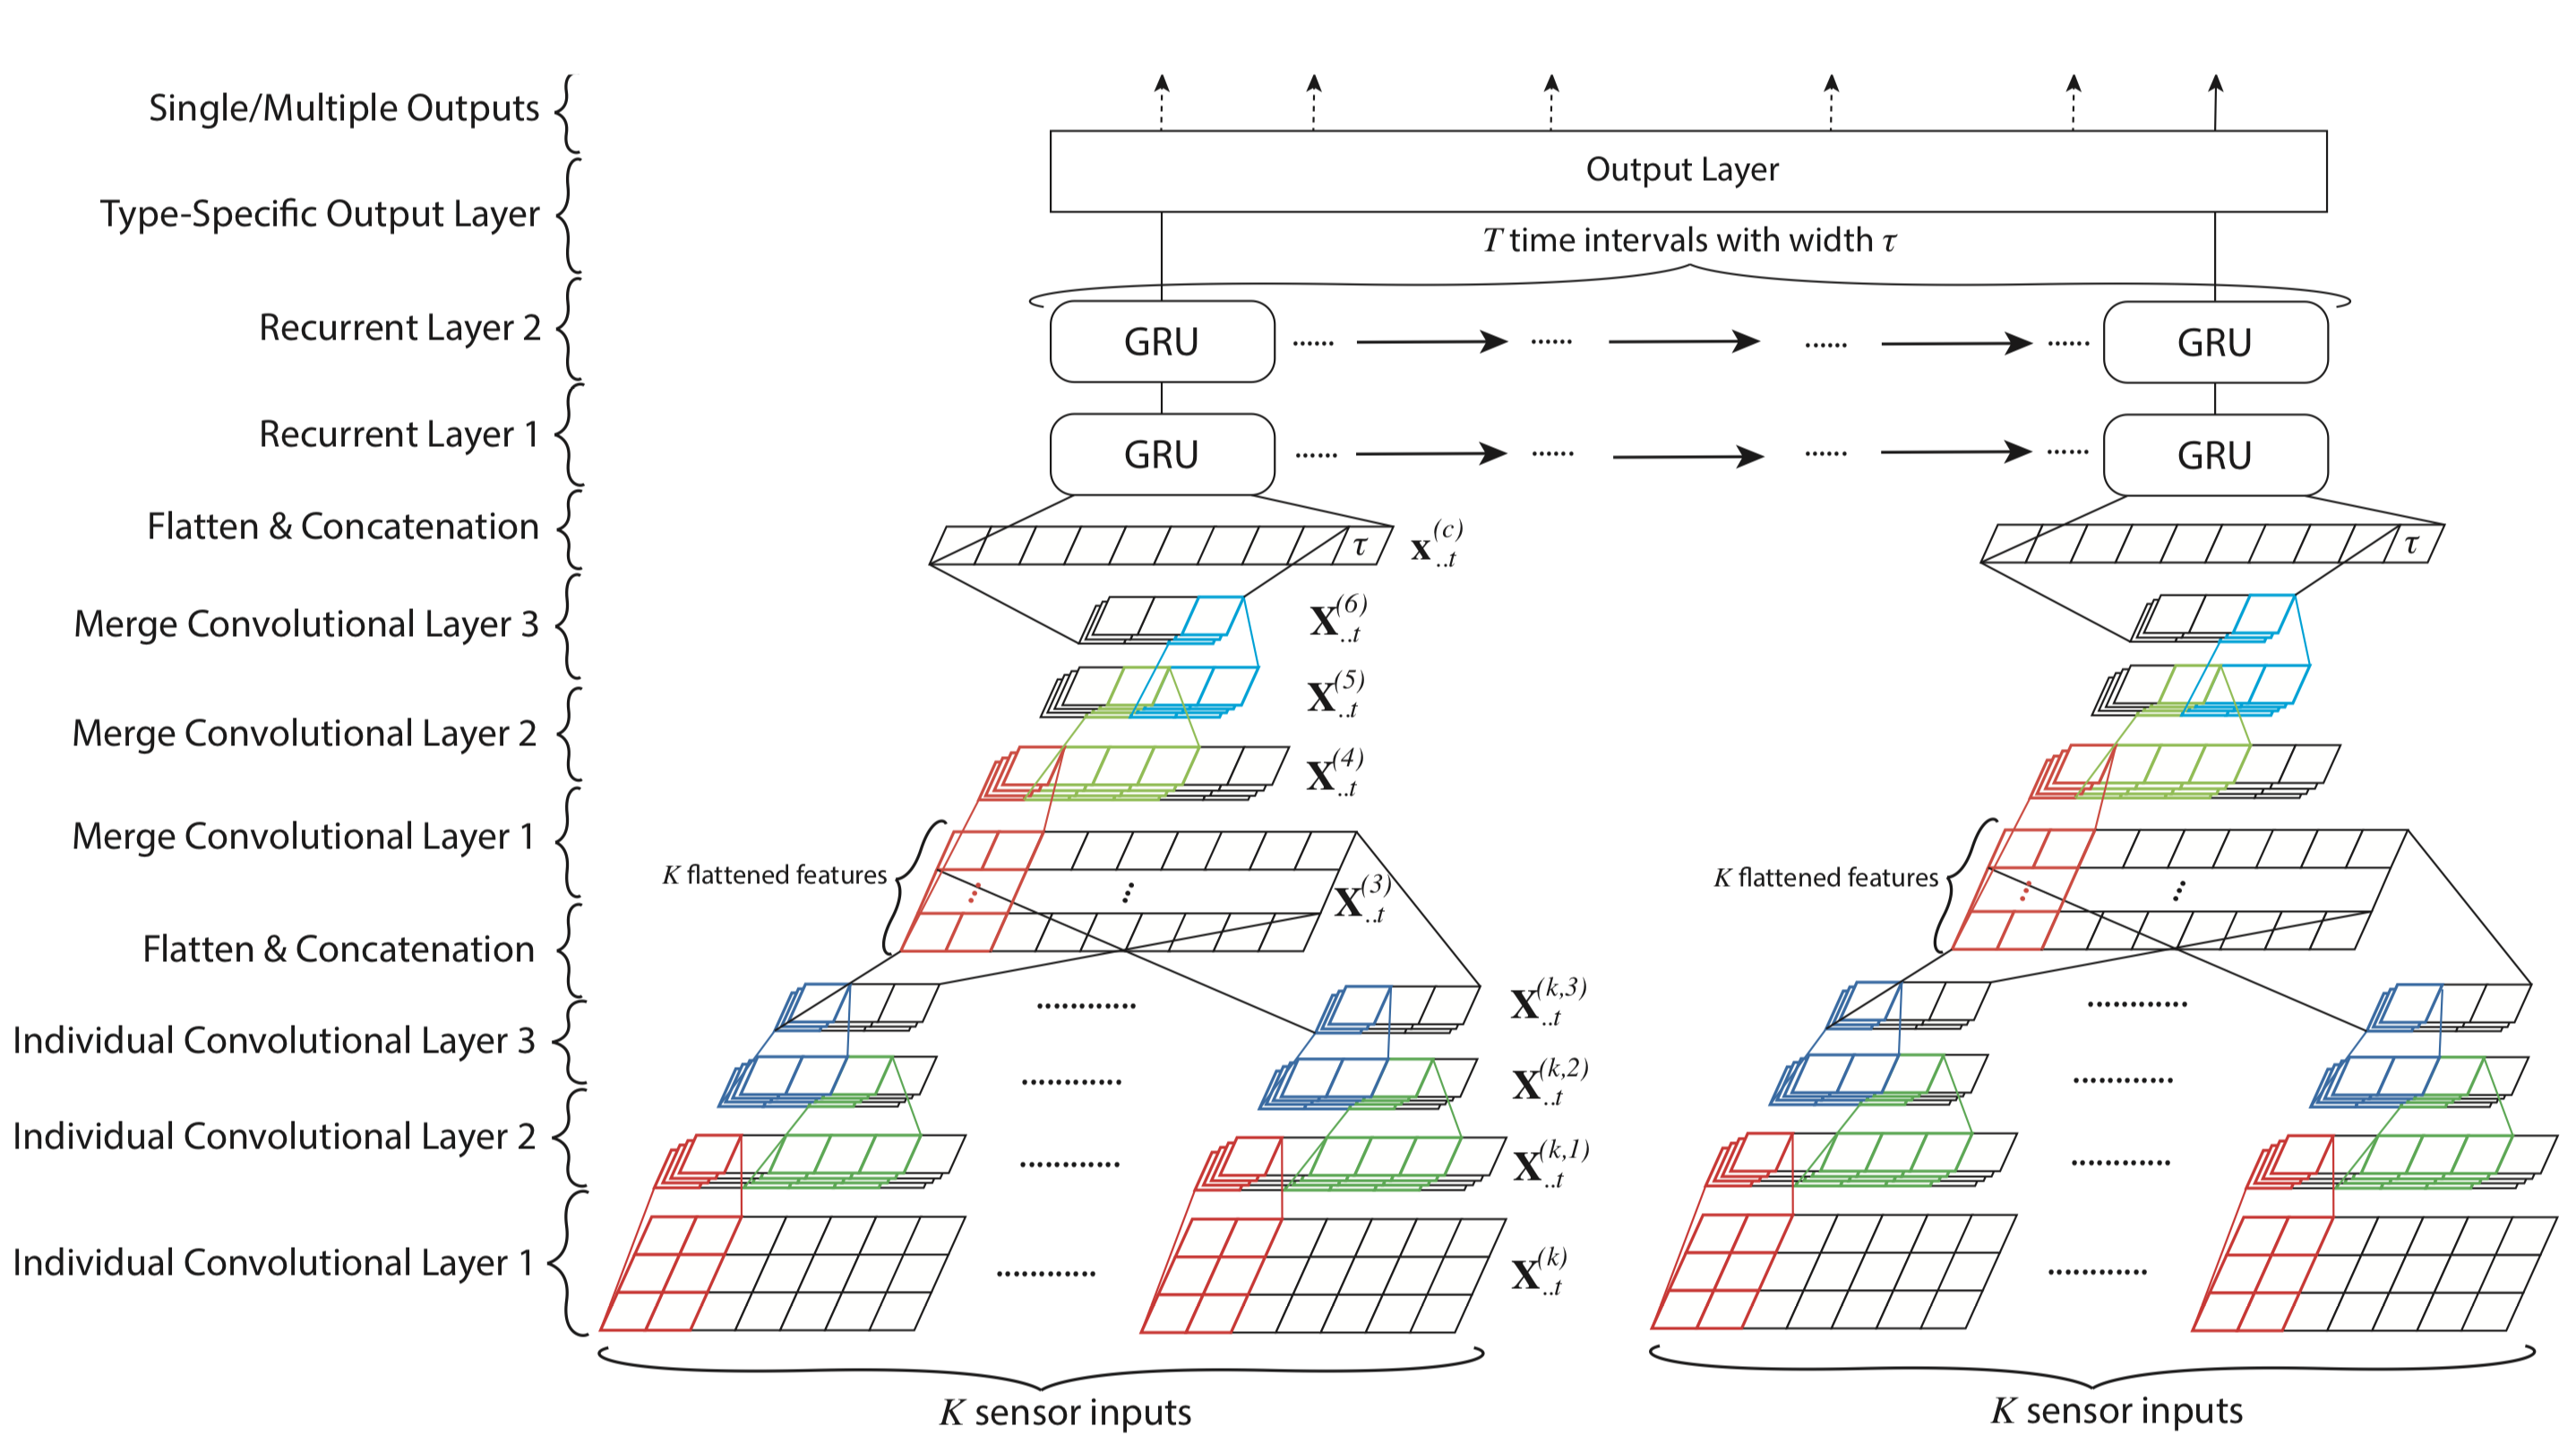
\includegraphics[width=0.6\textwidth]{deepsense}
\caption{DeepSense Architecture (\cite{yao2017deepsense})}
\label{fig:ds}
\end{figure}
A closer study of literature on sensor fusion architectures reveals that the evaluations however fail to present improvements that are statistical significant to support multiple sensors over a single sensor. In addition there is opportunity to improve on informed selection of sensors/features and noise reduction.  

\subsection{Attention}
Attention in deep models are mainly explored in the context of natural language processing but also seen in image processing to improve performance. 
They are a useful mechanism to optimise the manner in which features are attended upon for feature embedding.
In essence they provide a means to select features according to context as part of model learning.

\citeasnoun{mnih2014recurrent} introduce an attention mechanism with RNN to adaptively select regions from an input image or sequences from video. They mimic the human retina functionality by learning to focus on a selected region of the image. This selected area is learnt by the attention function, and the area outside this focus is considered as being blurred. Specifically the attention model is used to manage the area of of focus at input by updating the attention model based on feedback from the softmax output. 

Attention has also been applied with CNN architectures for Visual Question Answering tasks by ~\citeasnoun{chen2015abc}. Here unlike with RNNs the attention is used to influence the output from convolutions that are being learnt, by employing a number of convolution kernels on feature embeddings of an image to highlight the desired features for a given query embedding. This research interprets attention as selecting desirable convolution kernels per each query embedding and this approach outperforms the state of the art Bag-of-word methods and vanilla CNN or LSTM methods. 

In other related work attention has also been used to directly influence the the generation of the convolutional features~\cite{yin2015abcnn}. This provides an elegant means to influence one or more layers and has been successfully applied to NLP tasks to learn mutual influences between adjacent sentences for a given task. A Siamese Neural Net learns sentence similarities with a similarity-based attention matrix at each abstraction layer. Compared to \citeasnoun{chen2015abc}, this approach embed attention in to convolution layers. 

\subsection{Learning Paradigms}
In this section we detail three learning methodologies, each exploring different aspects of training machine learning models. We plan to explore these learning paradigms as needed in future in the context of  exercise classification and quality assessment. 

\subsubsection{Privileged Learning}
Privileged Learning (PL) mimics how humans learn with a teacher. In a learning environment teacher provides student with explanations, comments and examples but when tested student has to rely on what they learned. \citeasnoun{vapnik2009new} adapt this concept as an additional feature space (Privileged Information) that guarantees near perfect classification, but only available when the model is training. Defining Privileged Information (PI) is domain specific hence adaptable to many machine learning tasks.

\citeasnoun{chen2017training} use PI to minimize correlations between convolution functions. After learning feature representation for an input they suppress the background features using privileged knowledge, thus allowing the model to learn more foreground features desirable for classification. 

\citeasnoun{shi2017learning} attempt HAR with depth sequences for RNN with PI. Previous work involved with RNN and depth sequences required hand crafted features such as skeleton information which is a computationally expensive task. In this research they use Skeleton information as PI at training time and train a network for multiple tasks. First task is responsible for classification of depth sequence and second task learns to generate skeleton from depth sequence. At test time they use generated skeleton from the network itself as input for the classification task. 

Above literature exhibit that PI is open to interpretation. It enables building robustness in to models to handle missing modalities in real-time which improves usability and efficient deployment. 

\subsubsection{Sequence to Sequence Learning (\textit{seq2seq})}\mbox{}\\
Sequence to sequence Learning is an significant application domain of RNNs, specifically LSTMs. The goal is to generate a sequence from another sequence by learning inter-dependencies with LSTMs. Most notable and common usage is language translation where \citeasnoun{sutskever2014sequence} introduces \textit{seq2seq} with English to French translation. Improving on \cite{sutskever2014sequence}, \citeasnoun{luong2015multi} introduces multi-task \textit{seq2seq} learning where multiple encoders and multiple decoders learn multiple tasks in the same recurrence architecture. They evaluate language translation tasks in multi-task \textit{seq2seq} model.

We are interested in exploring \textit{seq2seq} in generating sensor data streams which does not appear in literature but interesting avenue to explore given their powerful ability to learn inter-dependencies and generate sequences. 

\subsubsection{Curriculum Learning}
Curriculum learning was first introduced by \citeasnoun{bengio2009curriculum} as defining a curriculum strategy for training a network. They adapt from human learning process where we start with simple examples and build up complexity. The curriculum strategy is open to interpretation decided by the application context.

\citeasnoun{havaei2016hemis} introduce a robust deep model to handle missing image modalities at test time by training the model with pseudo-curriculum training for medical imaging. All modalities were used as input in early epochs and then a random number of modalities were dropped from input for a given training instance enabling model to adapt to missing modalities. 

This methodology can be interpreted as a different perspective of PL as well where learning is interpreted as series of tests. 

\subsection{Exercise Quality}
Providing performance assessment is important in a digital intervention to maintain quality. but it is a subjective process. Performance quality of an exercise can be defined as how much actual execution deviates from correct execution of the exercise performed under the supervision of a physiotherapist. Measuring the deviation is open to interpretation and there is a lack of research in this area. Existing literature suggests performing classification on hand crafted features is the most explored method for determining quality of exercise. 

\citeasnoun{chen2013rehabilitation} is a notable publication on this area. Their data set consist of instances from both correct and incorrect performance of the exercises recorded with three accelerometers. Sensors were strategically placed on body to calculate angles of the body parts and with FFT features they classified type and correctness. In this research, correctness is modelled as binary classification task and provided in hindsight. 

\citeasnoun{velloso2013qualitative} model quality as a multi class classification task where one class represent correct execution while are different types of wrong executions. They also implement a rule based model where an execution will be matched against a set of rules derived from correct model. Rule-based approach out performs classification approach in their experiments and able to isolate the error to a single rule. 

Locating the problems within the sequence to provide meaningful feedback in real-time is a desirable feature in a qualitative evaluation and \citeasnoun{velloso2013qualitative} achieve with rule based system. But rule based system has many drawbacks such as need for expert knowledge, expense of maintenance and less generalizability. In addition above classification systems use hand crafted features and there is no evidence seen in literature exploring the advantages of deep models to address this task to our knowledge. 
